\section{Optimizing Pointwise Convolution}
\label{sec:pwconv}
In this section, we demonstrate the workflow of our dynamic blocking strategy as shown in Figure \ref{fig:pwworkflow} and Algorithm \ref{algo:pwalgo}. 
The whole workflow consists of two stages. 

In the first stage, our approach operates in a top-down fashion. 
We use a 3-level hierarchical partitioning method to decompose the output into three levels of tiles, including block level tiles, warp level tiles and thread level tiles. 
There are two main considerations when decomposing the output. First, how tiles are arranged in its upper level tile, and second, the height and width of each tile with the specified layout.

In the second stage, we calculate the exact height and width of thread level tiles. 
Given the number of output elements in each tile and hardware resources constraints, we iterate over all possible configurations of tile height and width of each level and choose the configuration that maxmize the performance most.

Now we give a detailed description of how each stage works.
\subsection{3-Level Hierarchical Partitioning}
In order to make it easier to understand the workflow of this stage, we first describe two important constant parameters and how we determine their values.

The first parameter is the number of warps in a thread block, denoted as $Warp_{num}$.
In order to determin the warp number, we need to consider: (1) small warp number will decrease the opportunity to hide the memory access latency at the warp level;
(2) large warp number will dcrease the number of thread blocks and may lead to SM underutilization.
Baed on both considerations, we decide to set $Warp_{num}=4$.
In our experiments, this value is good enough to provide a satisfied performance.

%this may not be important as i think
The second parameter is the number of thread blocks that can run concurrently on an SM.
We use two values, 2 and 4, for this parameter, denoted as $Block_{num}=\{2, 4\}$. 
There are two reasons for these choices: 
(1) when $Block_{num}=1$ and $Warp_{num}=4$, there are only 4 warps in an SM. 
As each thread can use up to 256 registers, a thread block can use at most $4*32*256=32768$ registers, which is only half of 65536 registers of an SM.
To avoid wasting hardware resources, we set $Block_{num}>1$; 
(2) when partitioning the output with the configuration of 4 thread blocks per SM, we encounter cases in which 5 or 6 thread blocks are actually running concurrently on an SM. 
This is because in some cases, each thread block requires very few hardware resources and more than 4 thread blocks can run concurrently on one SM.
Therefore, when searching for the best configurations, we only need $Block_{num}=\{2,4\}$.

Now we demonstrate the workflow of our 3-level hierarchical partitioning.
In Figure \ref{fig:pwworkflow}, we show two logical layouts of output, $F_N$ and $I_N \times I_H \times I_W$ represent the filter and input dimensions of the output respectively.
In the first level, we partition the output based on the number of filters, $F_N$.
When $F_N \ge 48$, we choose layout \textbf{\emph{L1}} and distribute filter channels across threads of the same warp. 
Otherwise, we choose layout \textbf{\emph{L2}} and distribute input channels.
The rationale behind this choice can be described as follows. 
The number of filters, $F_N$, is fixed once the structure of a CNN is determined. 
But the dimension of the input will be affected by the batch size, $I_N$, during inference and training.
For the sake of simplicity, we design and implement our dynamic partitioning startegy to utilize layout \textbf{\emph{L1}} whenever there are enough filters to be distributed across threads.
We will explain later in this section why we choose 48 as the boundry of layout \textbf{\emph{L1}} and \textbf{\emph{L2}}.

Next, we partition both layouts of output into block tiles along the filter dimension. 
For the layout \textbf{\emph{L1}}, we halve the filter dimension if $F_N \geq 512$. 
The reason is that if we let each block tile process excessive amount of filters, there will be few options for channel number{\color{red}explain this in previous text} when distributing channels across threads. 
This may cause our dynamic partitioning startegy to find a sub-optimal configuration for pointwise convolution.
For the layout \textbf{\emph{L2}}, we halve the filter dimension if $F_N \geq 24$.
Last, we halve both dimensions of each block tile and generate $2 \times 2$ warp tiles. The height and widht of a warp tile are represented as $Warp_H$ and $Warp_W$ respectively.

\subsection{Distribute Channels Over Threads}
In this stage, we iterate over all candidate combinations of channel count and $Warp_H$, and select the combination that leads to optimial SM utilization and arithmetic intensity.

First, we describe how to determine the candidates for channel count and $Warp_H$ with layout \textbf{\emph{L1}}. Layout \textbf{\emph{L2}} has a similar process.
Assume that we distribute 8 channels across threads, which means that 8 threads will load 8 channels of the filter into registers. 
Therefore, 32 threads of a warp can load 8 channels of $32/8=4$ filters  at the same time.
To increase the arithmetic intensity, we need to distribute channels over threads. The most important cosideration is how to determine the number of threads that collaborate one output element. We use 6 values for the channel count, denoted as $C_{num}=\{1,2,4,8,16,32\}$. 
Figure \ref{fig:pwworkflow} demonstrates that we use 8 threads to calculate 8 channels of one output element at the same time. 

For each option of $C_{num}$, we calculate how many elements a warp can process at the same time, denoted as $Ele_{count}=32/C_{num}$. 
Then we get the number of elements each thread needs to process, denoted as $T_{num}=WarpTile_W/Ele_{count}$.
When calculating the same amount of output elements, square blocking uses the least load instructions. 
Therefore, we try to set the height of the thread tile to $T_{num}$.
First, we compare the value of $T_{num}$ with $InitWarp_H$.
If $T_{num}>InitWarp_H$, meaning there is not enough output elements to construct a square tile, we set $Warp_H=InitWarp_H$, otherwise, set $Warp_H=T_{num}$.
Then update $Block_H=2*Warp_H$.

Now we describe the constraints on registers and shared memory. Based on $Block_{num}$, we calculate the number of registers each thread can use and the size of shared memory each thread block can use, denoted as $Limit_R=65536/(Block_{num}*4*32)$ and $Limit_S=64*1024B/Block_{num}$ respectively.
The constraints can be formulated as follows:
\begin{equation}\nonumber
R_{o}=WarpTile_H*T_{num},R_{tmpf}=\frac{C_{num}*BlockTile_W}{128}
\end{equation}
\begin{equation}\nonumber
R_{f}=WarpTile_H,R_{i}=T_{num},R_{tmpi}=\frac{C_{num}*BlockTile_H}{128}
\end{equation}
\begin{equation}
R_{o}+R_{i}+R_{f}+R_{tmpf}+R_{tmpi}+const \leq Limit_R
\end{equation}
\begin{equation}
(BlockTile_H+BlockTile_W)*C_{num}*4*2 \leq Limit_S
\end{equation}
\begin{figure*}
	\centering
    %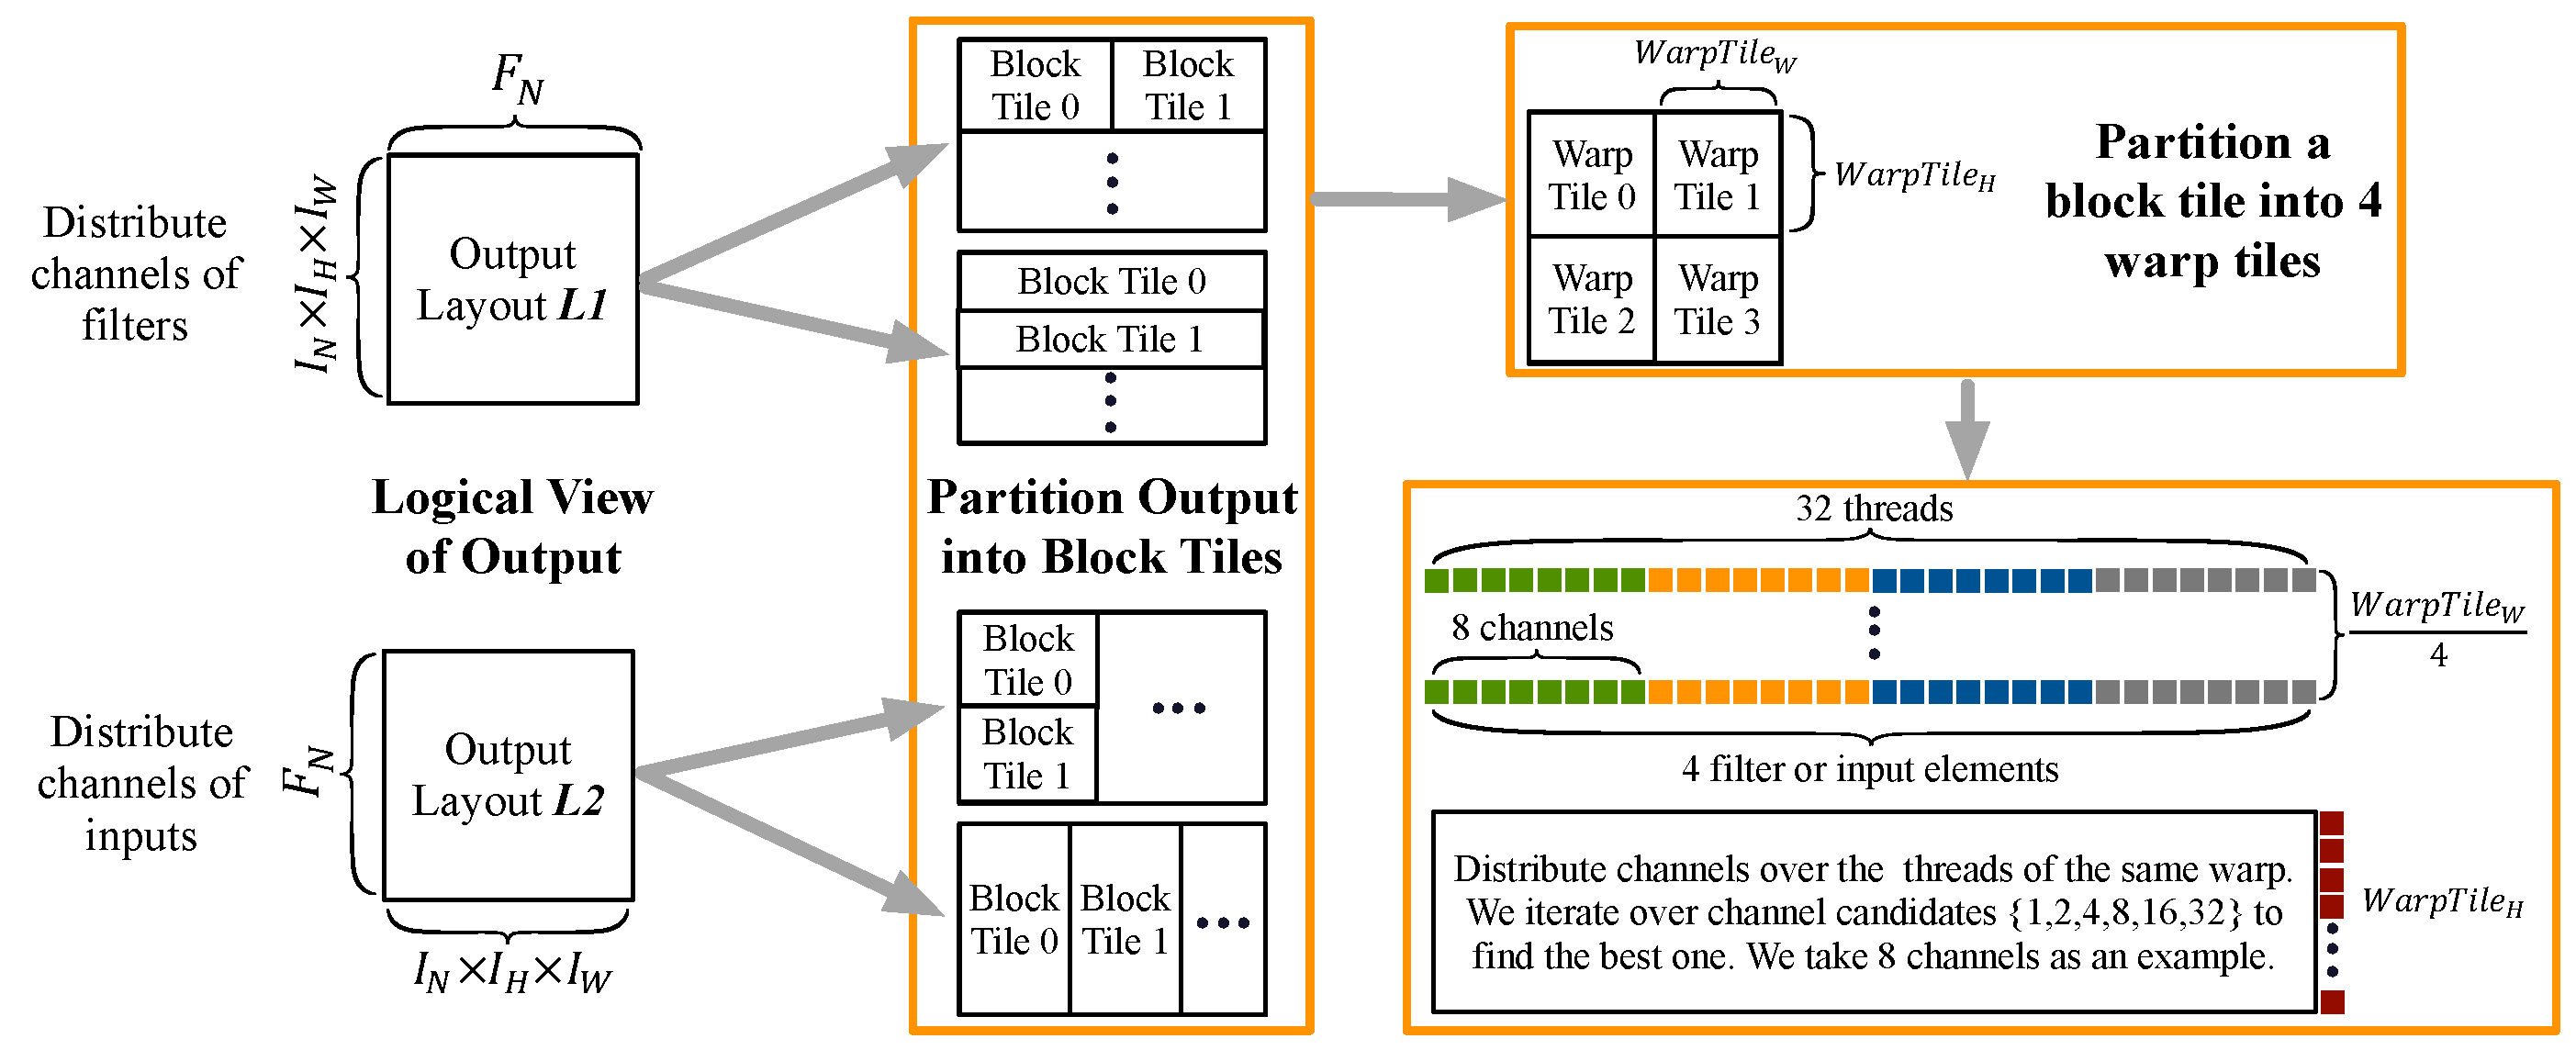
\includegraphics[width=\columnwidth]{./figure/pwworkflow1.eps}
    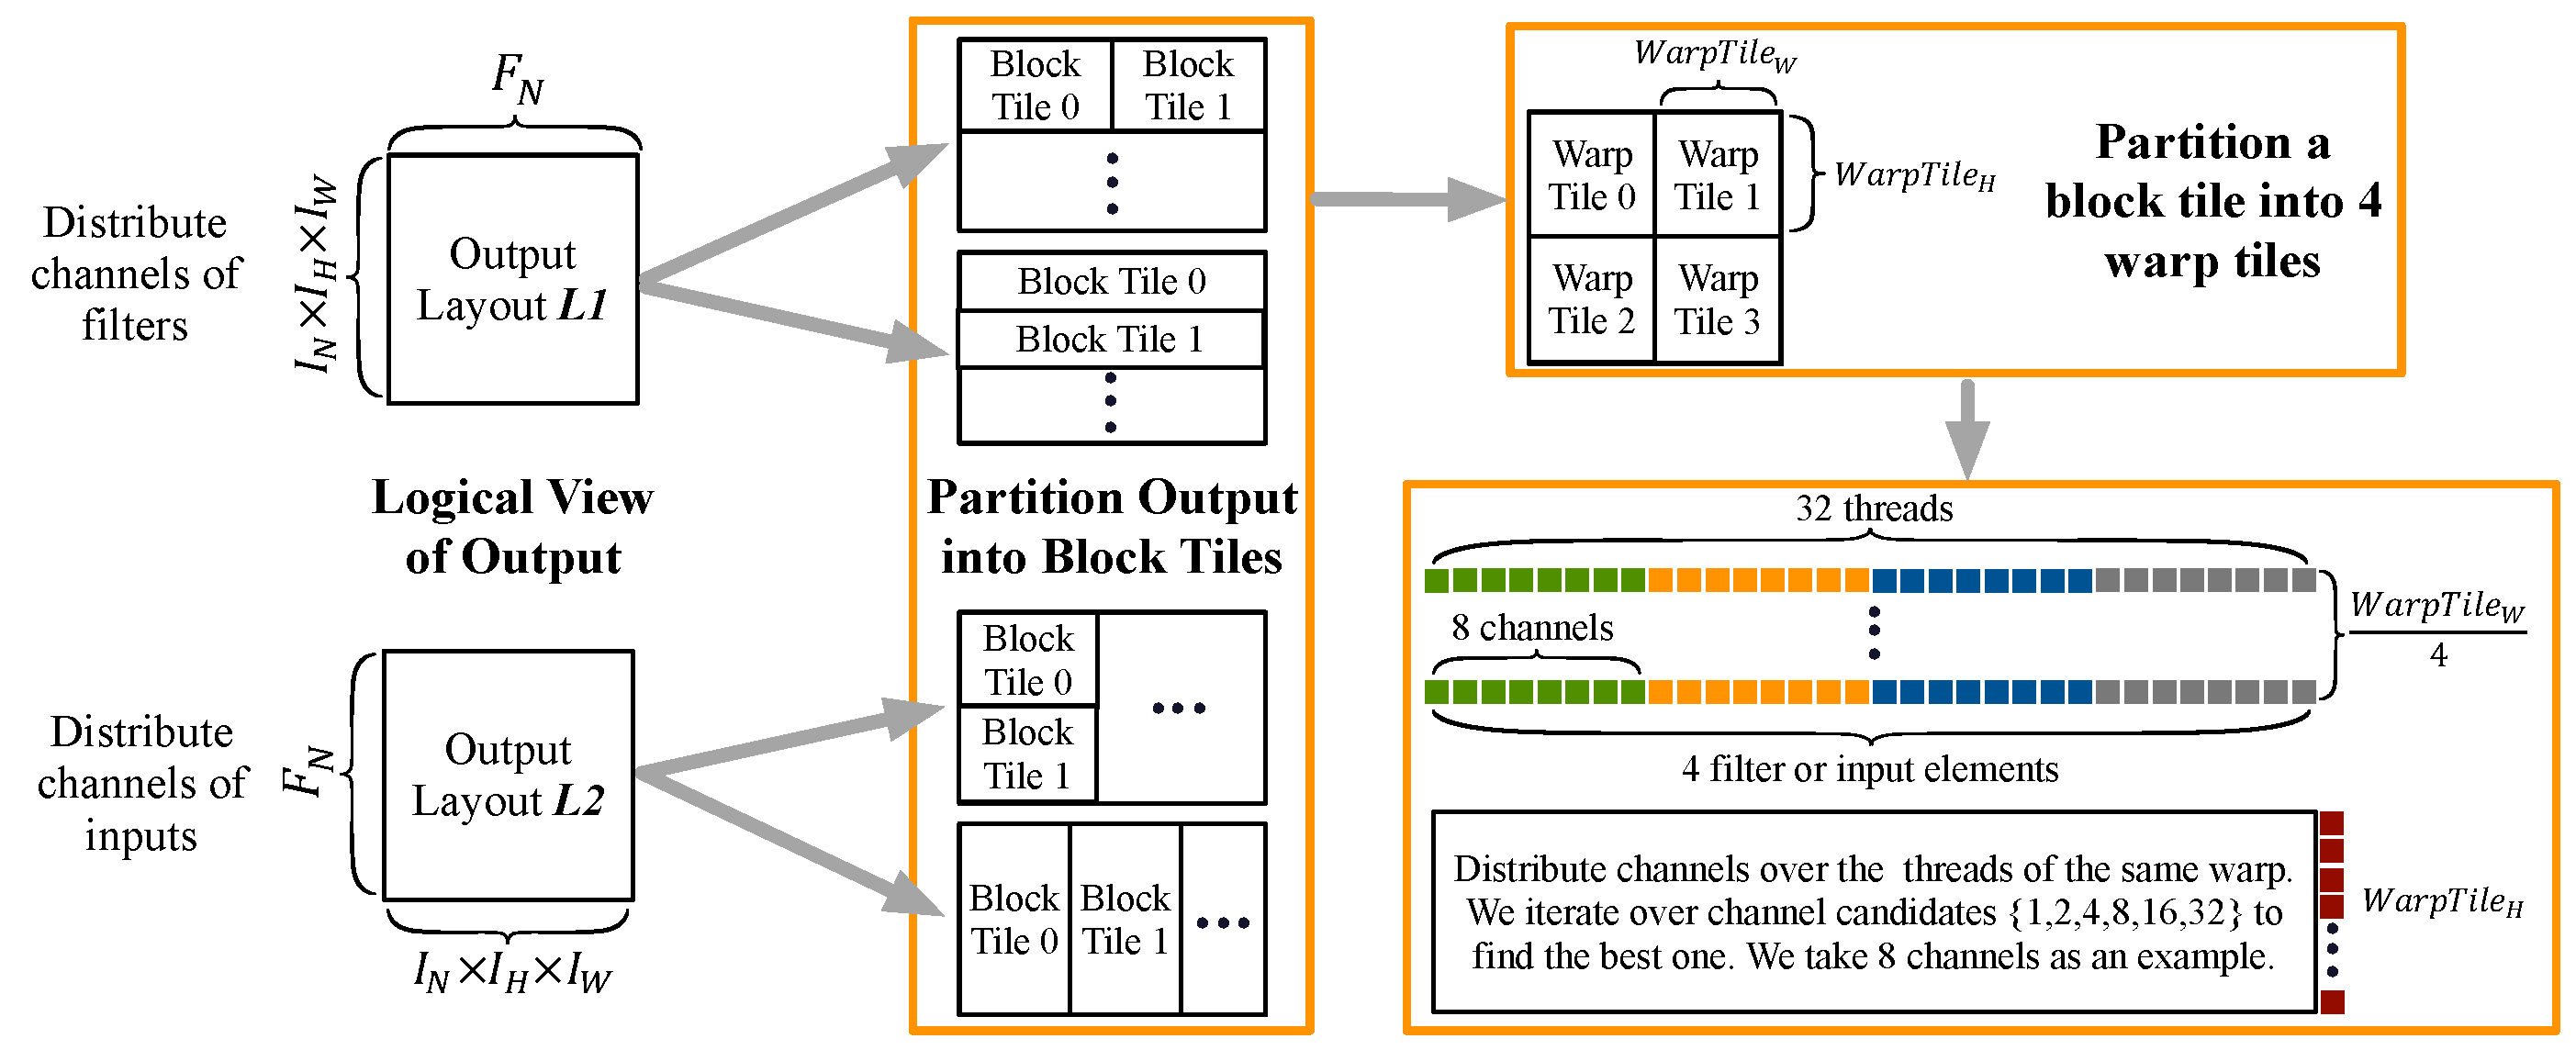
\includegraphics[width=0.95\textwidth,height=7cm]{./figure/pwworkflow1.eps}
    \caption{} \label{fig:pwworkflow}
\end{figure*}
\begin{algorithm}[t!]
    \small
        \KwIn{$I$, $F$}
        \KwOut{$O$}
        Calculate how many output elements one SM needs to process if we want to fully utilize GPU, denoted as $O_{sm}$\;
        \tcp{below codes are executed on CPU}
        \tcp{we have two options for block tile number, one SM contains 2 or 4 block tiles}
        \ForEach{block tile number of one SM}{
            Use $BlockTile_{count}$ to denote the number of block tiles resided on one SM\;
            \ForEach{block layout}{
                Calculate the width of a block tile, denoted as $BlockTile_W$\;
                $BlockTile_H = \frac{O_{sm}}{BlockTile_W * BlockTile_{count}}$\;
                \If{$BlockTile_H > 32$}{
                    $niter = BlockTile_H/32$\;
                    $BlockTile_H = 32$\;
                }
                $WarpTile_H=\frac{BlockTile_H}{2}$\;
                $WarpTile_W=\frac{BlockTile_W}{2}$\;
                \tcp{there are 6 choices for channel count, 1,2,4,8,16,32}
                \ForEach{channel count}{
                    Use $C_{count}$ to denote how many threads are uesed to calculate channels of the same output element.\;
                    $filter_{num} = \frac{32}{C_{count}}$\;
                    $filter_{num} = \frac{WarpTile_W}{filter_{num}}$\;
                    Calculate registers and shared memory usage under this configuration, and evaluate if the usage not exceeds the limit.\;
                    record the configuration with smallest register usage. 
                }
            }
        }
        \tcp{below codes are executed on GPU}
        All threads in a thread block cooperate to load the needed input and filter into shared memory\;
        $\_\_syncthreads()$\;
        \For{$iter \gets 0$ \KwTo $I_C$ By $C_{count}$}{
            load next $C_{count}$ channels for input and filter into registers\;
            load current channels of input and filter into registers\;
            calculate output elements\;
            write registers of next channels into shared memory\;
        }
        use segmented parallel reduce to get the final output elements and write the result to global memory\;
        \caption{Pointwise Convolution Optimization}
        \label{algo:pwalgo}
\end{algorithm}

We use two metrics, arithmetic intensity and thread block number, to select the best combinations. Two metrics are represented with notation $M_{A}$ and $M_{B}$, and can be calculated as follows:
\begin{equation}
    M_{A}=\frac{WarpTile_H*T_{num}*Iter}{R_{tmpf}+R_{tmpi}}
\end{equation}
\begin{equation}
    M_{B}=\frac{SM_H}{Block_H}*\frac{SM_W}{Block_W}*SM_{num}
\end{equation}

We first choose the best combination based on $M_{A}$, if two $M_{A}$ are close enough, then we choose the combination with smallest $M_{B}$. 